\subsection{Metodo del Gradiente Coniugato (naive)}
Il metodo del gradiente coniugato è un algoritmo per la risoluzione numerica di un sistema lineare la cui matrice sia simmetrica e definita positiva
 e consente di risolvere il sistema in un numero di iterazioni che è al massimo $n$.

La funzione $f$ da minimizzare è data dalla formula
  $f(x) = \frac{1}{2} ||Ax - b||_2^2 $, il cui gradiente $\nabla f$ è dato da
$\nabla f(x) = A^TAx - A^Tb  $.

Utilizzando il metodo del gradiente coniugato implementato dalla funzione \code{minimize}
 abbiamo calcolato la soluzione naive.

\begin{figure}[H]
  \centering
  \begin{subfigure}{0.9\textwidth}
    \centering
    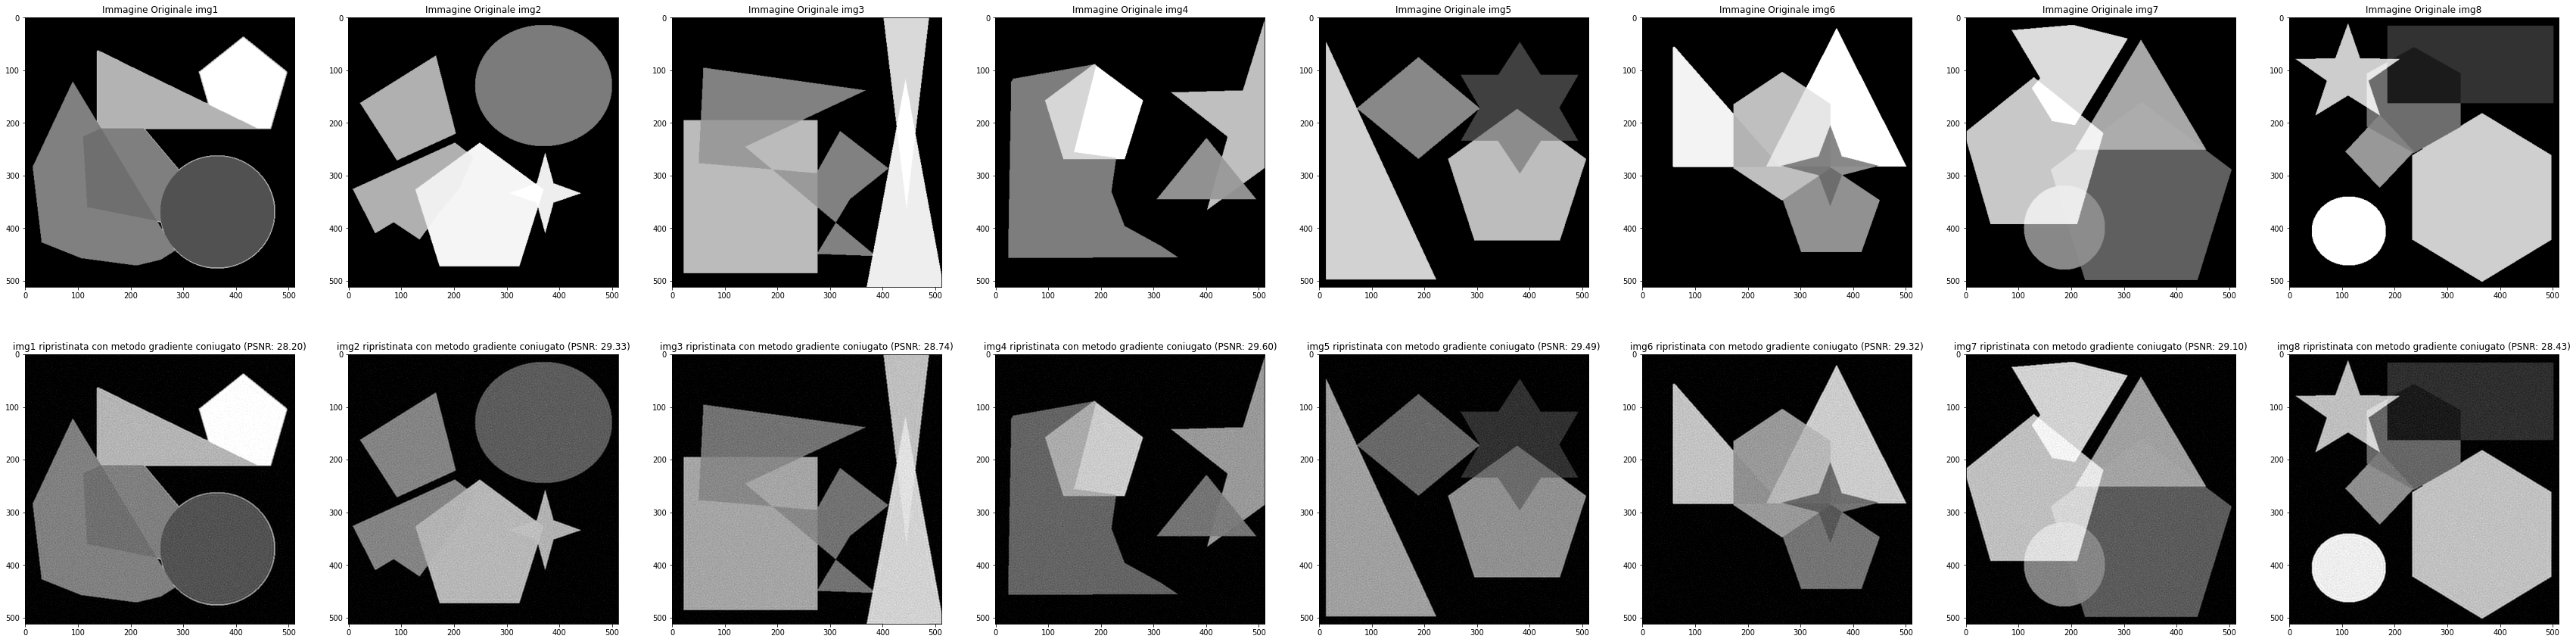
\includegraphics[width=0.9\textwidth]{imgRel/datasetconiugato.png}
    \caption{Immagini geometriche ripristinate}
    \label{fig:geomripristinate}
  \end{subfigure}

  \begin{subfigure}{0.5\textwidth}
    \centering
    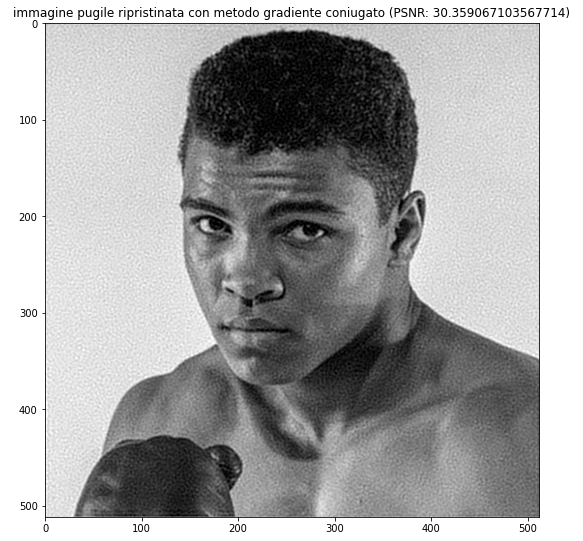
\includegraphics[width=0.6\linewidth]{imgRel/pugilemgc.png}
    \caption{Immagine fotografica ripristinata}
    \label{fig:pugilemgc}
  \end{subfigure}\hfill
  \begin{subfigure}{0.5\textwidth}
    \centering
    
\includegraphics[width=0.6\linewidth]{imgRel/giornalemgc.png}
    \caption{Immagine con testo ripristinata}
  \end{subfigure}
  \caption{Immagini analizzate ripristinate con il Metodo del Gradiente Coniugato}

  \centering
    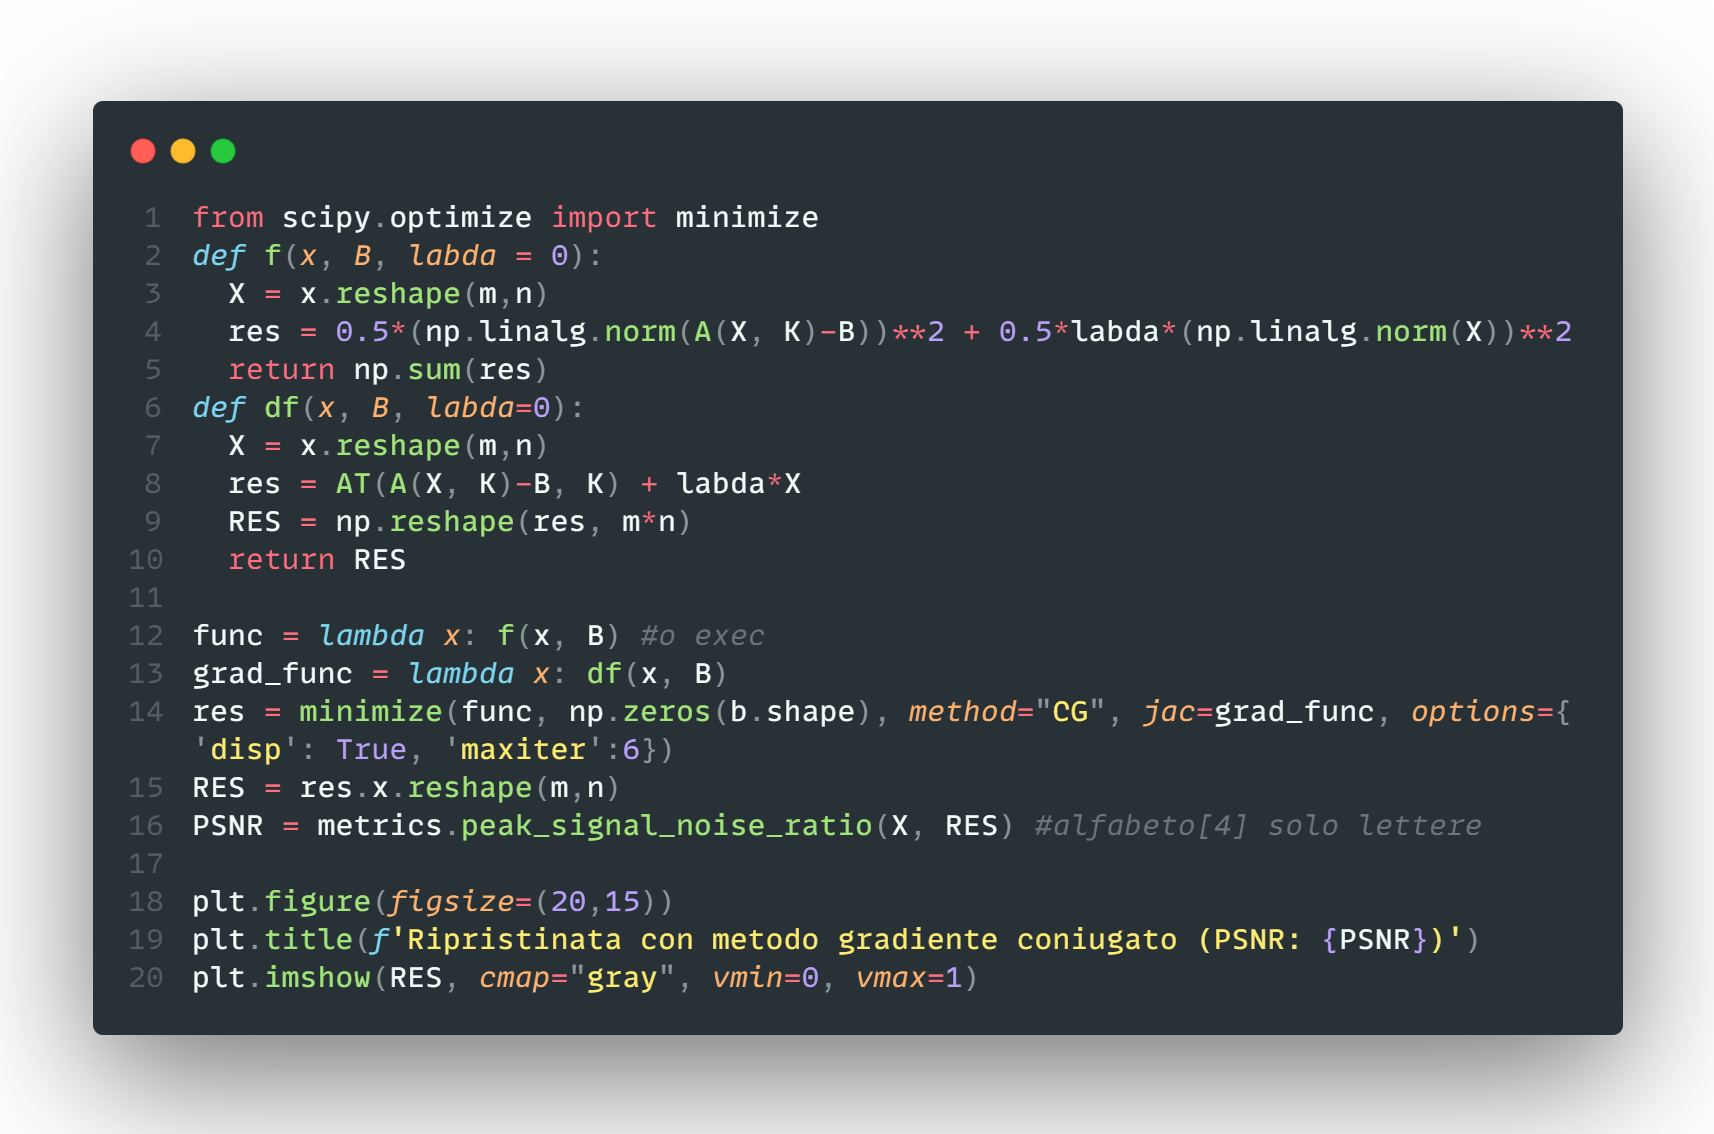
\includegraphics[width=0.6\textwidth]{imgCode/metGradCon.png}
    \caption{Codice Metodo del Gradiente Coniugato applicato ad una singola immagine}
    \label{fig:codeMGC}
\end{figure}

Con il metodo del gradiente coniugato abbiamo ripristinato le immagini, ottenendo un PSNR definitivamente superiore 
rispetto al PSNR dell'immagine corrotta iniziale.

Per esempio considerando l'immagine fotografica avremo che:\\
\textbf{Immagine ripristinata \ref{fig:pugilemgc}} PSNR: 30.359067\\
\textbf{Immagine corrotta \ref{fig:fotogrCorrotte7x7}} PSNR: 30.9049\\